\documentclass[twoside,11pt]{article}

% Any additional packages needed should be included after jmlr2e.
% Note that jmlr2e.sty includes epsfig, amssymb, natbib and graphicx,
% and defines many common macros, such as 'proof' and 'example'.
%
% It also sets the bibliographystyle to plainnat; for more information on
% natbib citation styles, see the natbib documentation, a copy of which
% is archived at http://www.jmlr.org/format/natbib.pdf

\usepackage{jmlr2e}
\usepackage{hyperref} % for clickable links
\usepackage{csvsimple} % for csv to table conversion
\usepackage{subfigure}
\usepackage{enumitem}
% Definitions of handy macros can go here

\newcommand{\dataset}{{\cal D}}
\newcommand{\fracpartial}[2]{\frac{\partial #1}{\partial  #2}}

% Heading arguments are {volume}{year}{pages}{submitted}{published}{author-full-names}

\jmlrheading{1}{2000}{1-48}{04/23}{Van Der Male}

% Short headings should be running head and authors last names

\ShortHeadings{Medical Insurance Fraud Detection}{Van Der Male}
\firstpageno{1}

\begin{document}

\title{Medical Insurance Fraud Detection}

\author{\name Aaron Van Der Male \email vandermale.a@northeastern.edu \\
       \addr Khoury College of Computer Science\\
       Northeastern University\\
       }

\editor{Aaron Van Der Male}

\maketitle


\section{Introduction}
Medical insurance fraud involves filing false or inaccurate insurance claims in an attempt to recieve undue insurance payouts.
In this project, a synthetic dataset of insurance claims is analyzed to distinguish fraudulent from legitimate insurance claims.
\\
\section{Objective}
The purpose of this project is to identify and score a machine learning classification model that can accurately classify insurance claims.
\section{Dataset}
 \href{htps://www.kaggle.com/datasets/beenusharma42/fraudlent-claim-in-healthcare}{A Kaggle Dataset}
 was analyzed. The csvs are joined in a pandas dataframe before processing:
 \begin{itemize}
    \item Train-1542865627584.csv: Contains provider numbers and value that shows if the provider is potentially fraudulent.
    \item Test-1542865627584.csv: Contains provider number.
    \item TrainBeneficiarydata-1542865627584.csv: Beneficiary data such as dob, race, gender, state, chronic condition, annual reimbursement amount, open annual deductible amount.
    \item TrainInpatientdata-1542865627584.csv
    \item TrainOutpatientdata-1542865627584.csv
    \item TestInpatientdata-1542969243754.csv
    \item TestOutpatientdata-1542969243754.csv
  \end{itemize}
\newpage


The dataset has 31 features that are to be analyzed. They are introduced in this section.
Figure 1 shows the data types of the features.
\begin{figure}[h]
    \center
    \csvautotabular{csv/dtypes.csv}
    \label{fig:dtypes}
    \caption{Feature Data Types}
\end{figure}
\newpage
A brief description of each feature is provided in Figure 2

\begin{figure}[h]
  \center
    \csvreader[
        tabular = {p{5cm} p{8cm} c}, % specify column widths
        head to column names,
        table head = \textbf{Name} & \textbf{Description} \\
        ]
        {csv/desc.csv}{}
        {\Feature & \Description}
  \label{fig:descr}
  \caption{Feature Names and Descriptions}
\end{figure}


% Understanding the Dataset 
\newpage
\section{Understanding the Dataset}

The frequency of features in the dataset is explored. Figure 3 and 4 depict
the amount of data collected along state, gender, and racial divisions. The histograms
in figures 5, 6 and 7
 characterize the differences between the fraudulent and normal claims.
\begin{figure}[h]
  \centering
  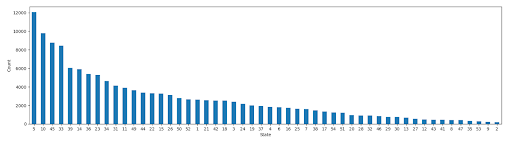
\includegraphics[width=\textwidth]{./img/sdist.png}
  \caption{State Distribution}
  \label{fig:grdist}
\end{figure}

\begin{figure}[h]
  \centering
  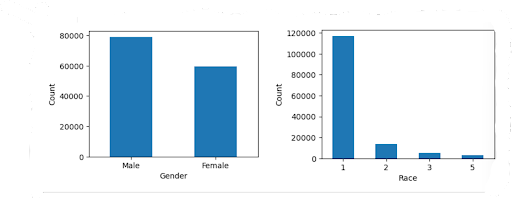
\includegraphics[width=\textwidth]{./img/grdist.png}
  \caption{Gender and Race Distribution}
  \label{fig:sdist}
\end{figure}

\begin{figure}[bp!]
  \centering
  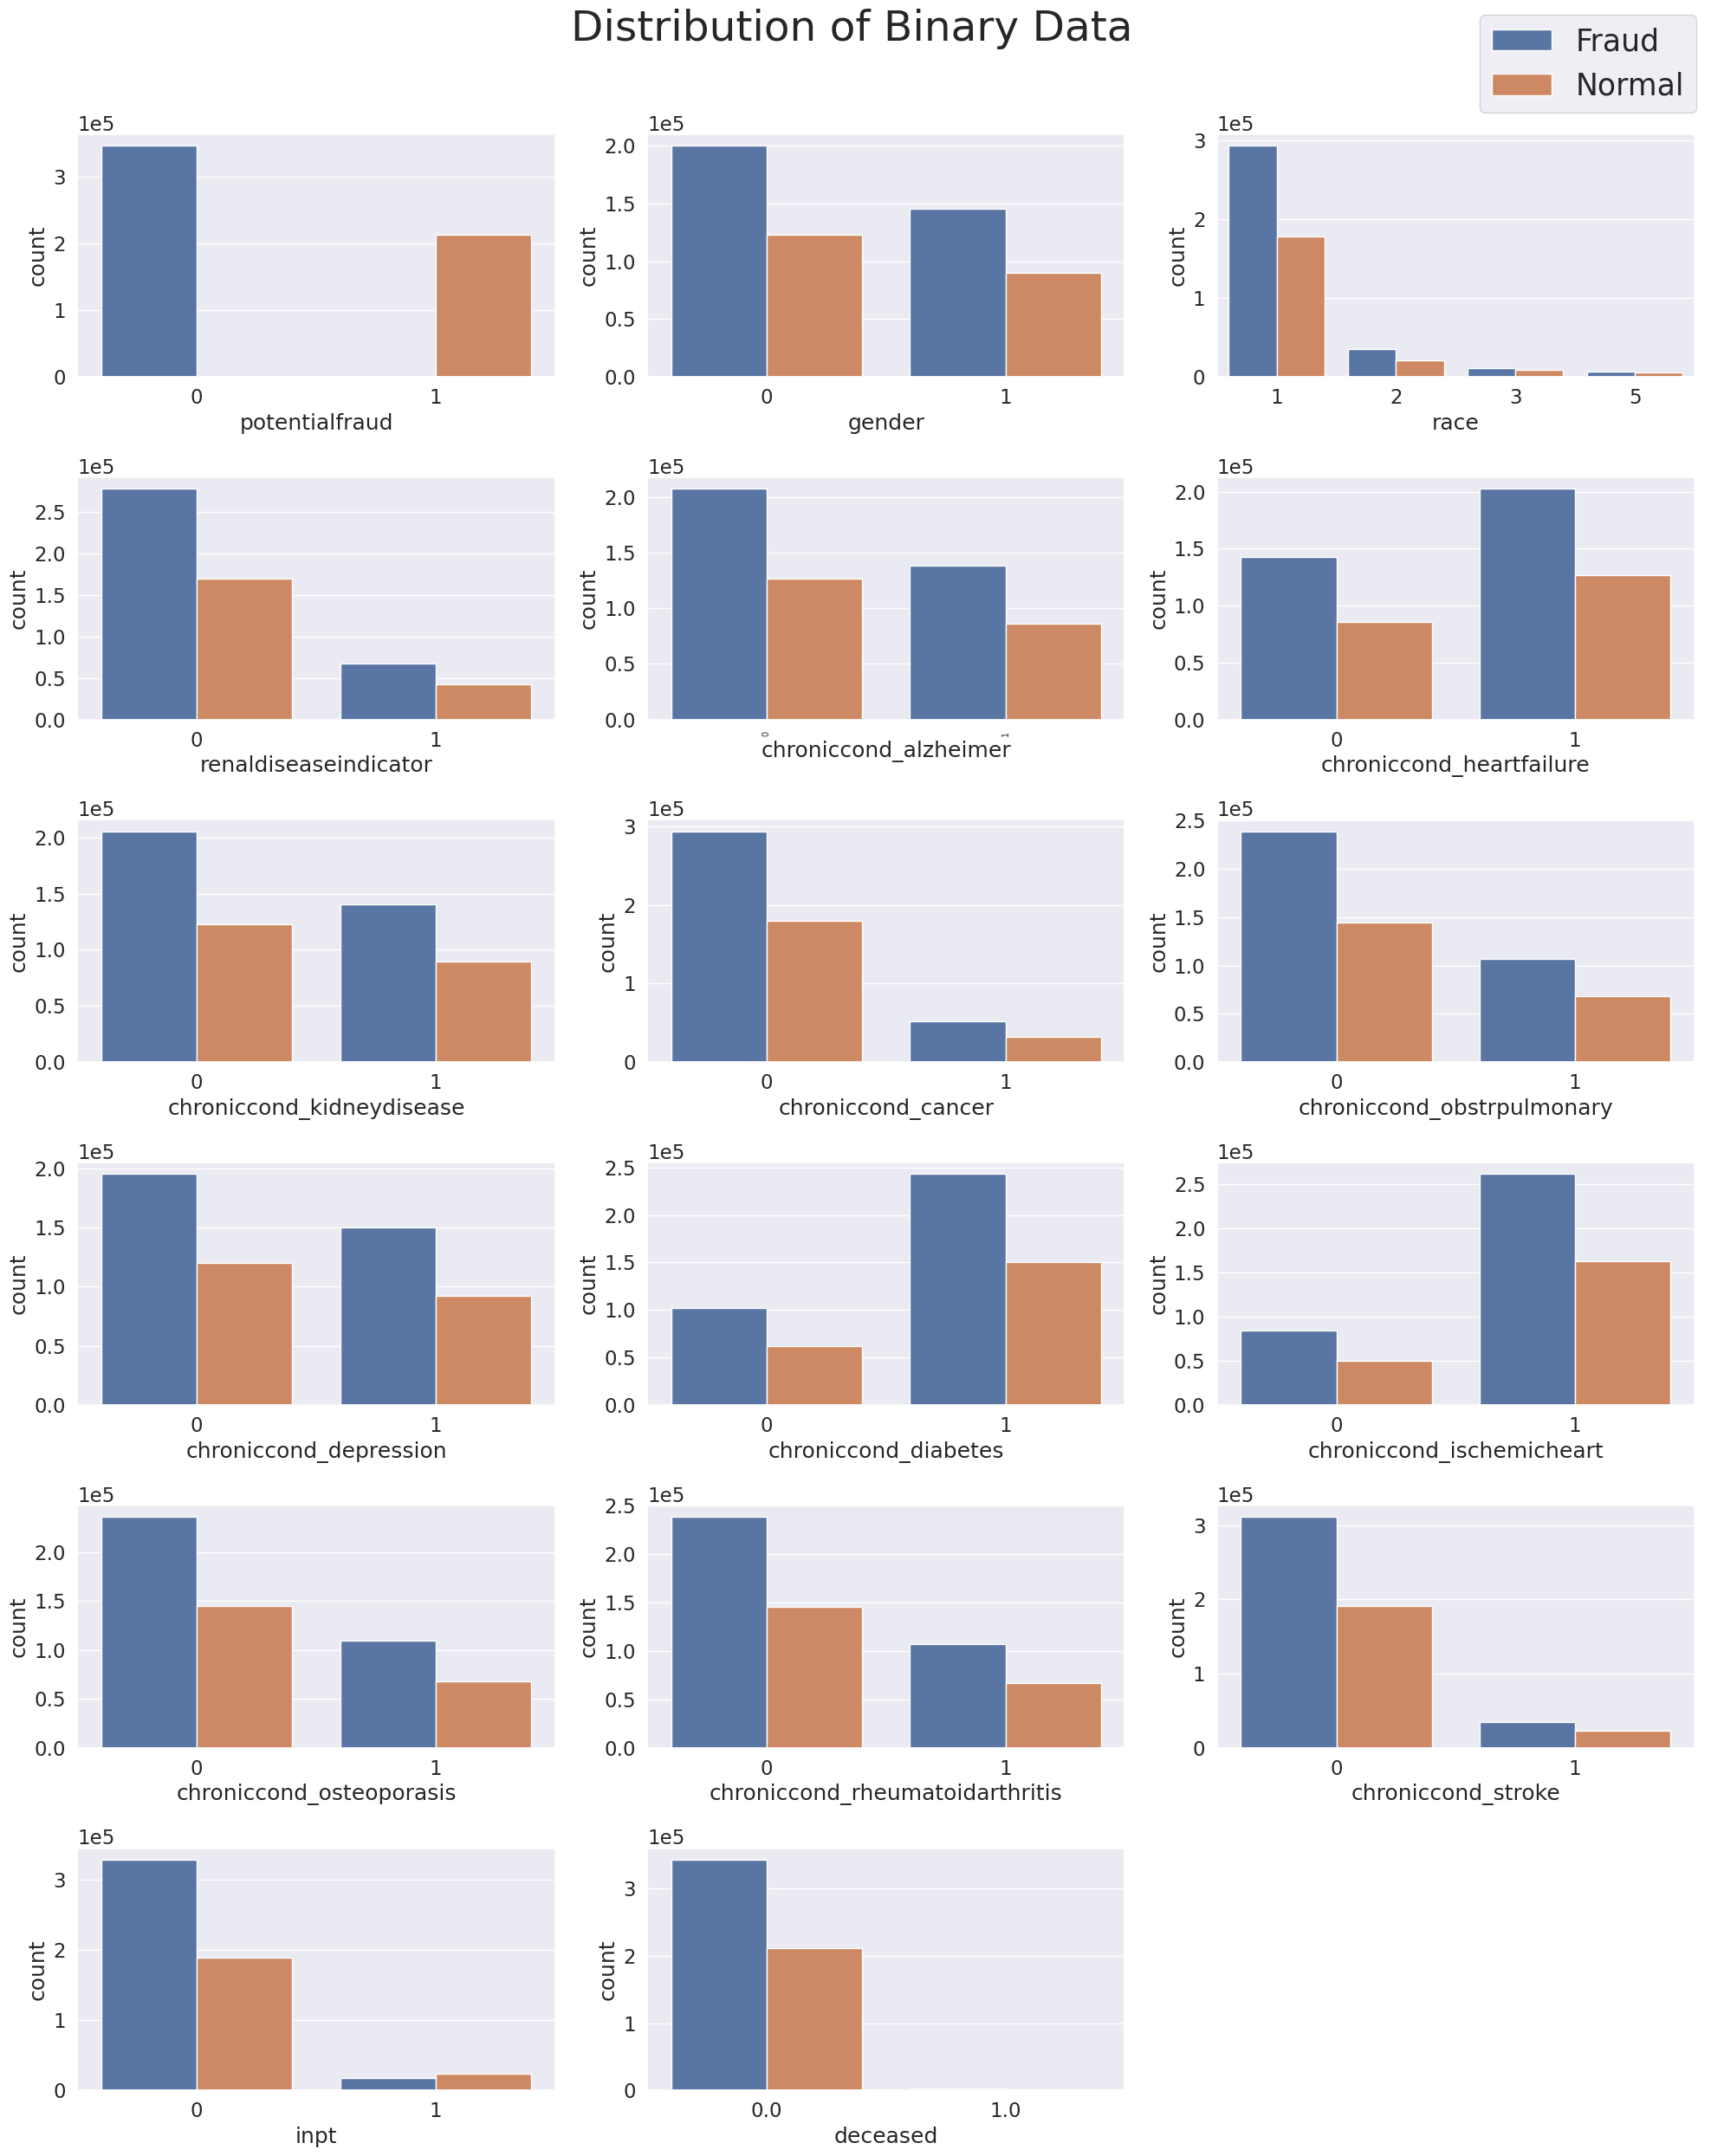
\includegraphics[width=\textwidth]{./img/binary.png}
  \caption{Distribution of Binary Data}
  \label{fig:binary}

\end{figure}
\begin{figure}[bp!]
  \centering
  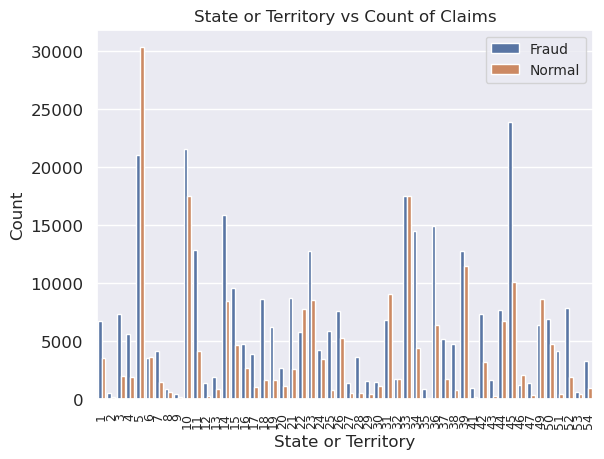
\includegraphics[width=\textwidth]{./img/state.png}
  \caption{Distribution of State or territory Data. The 
  names of the states are not
  provided with this dataset, and the data are instead identified with a number.}
\end{figure}

\begin{figure}[bp!]
  \centering
  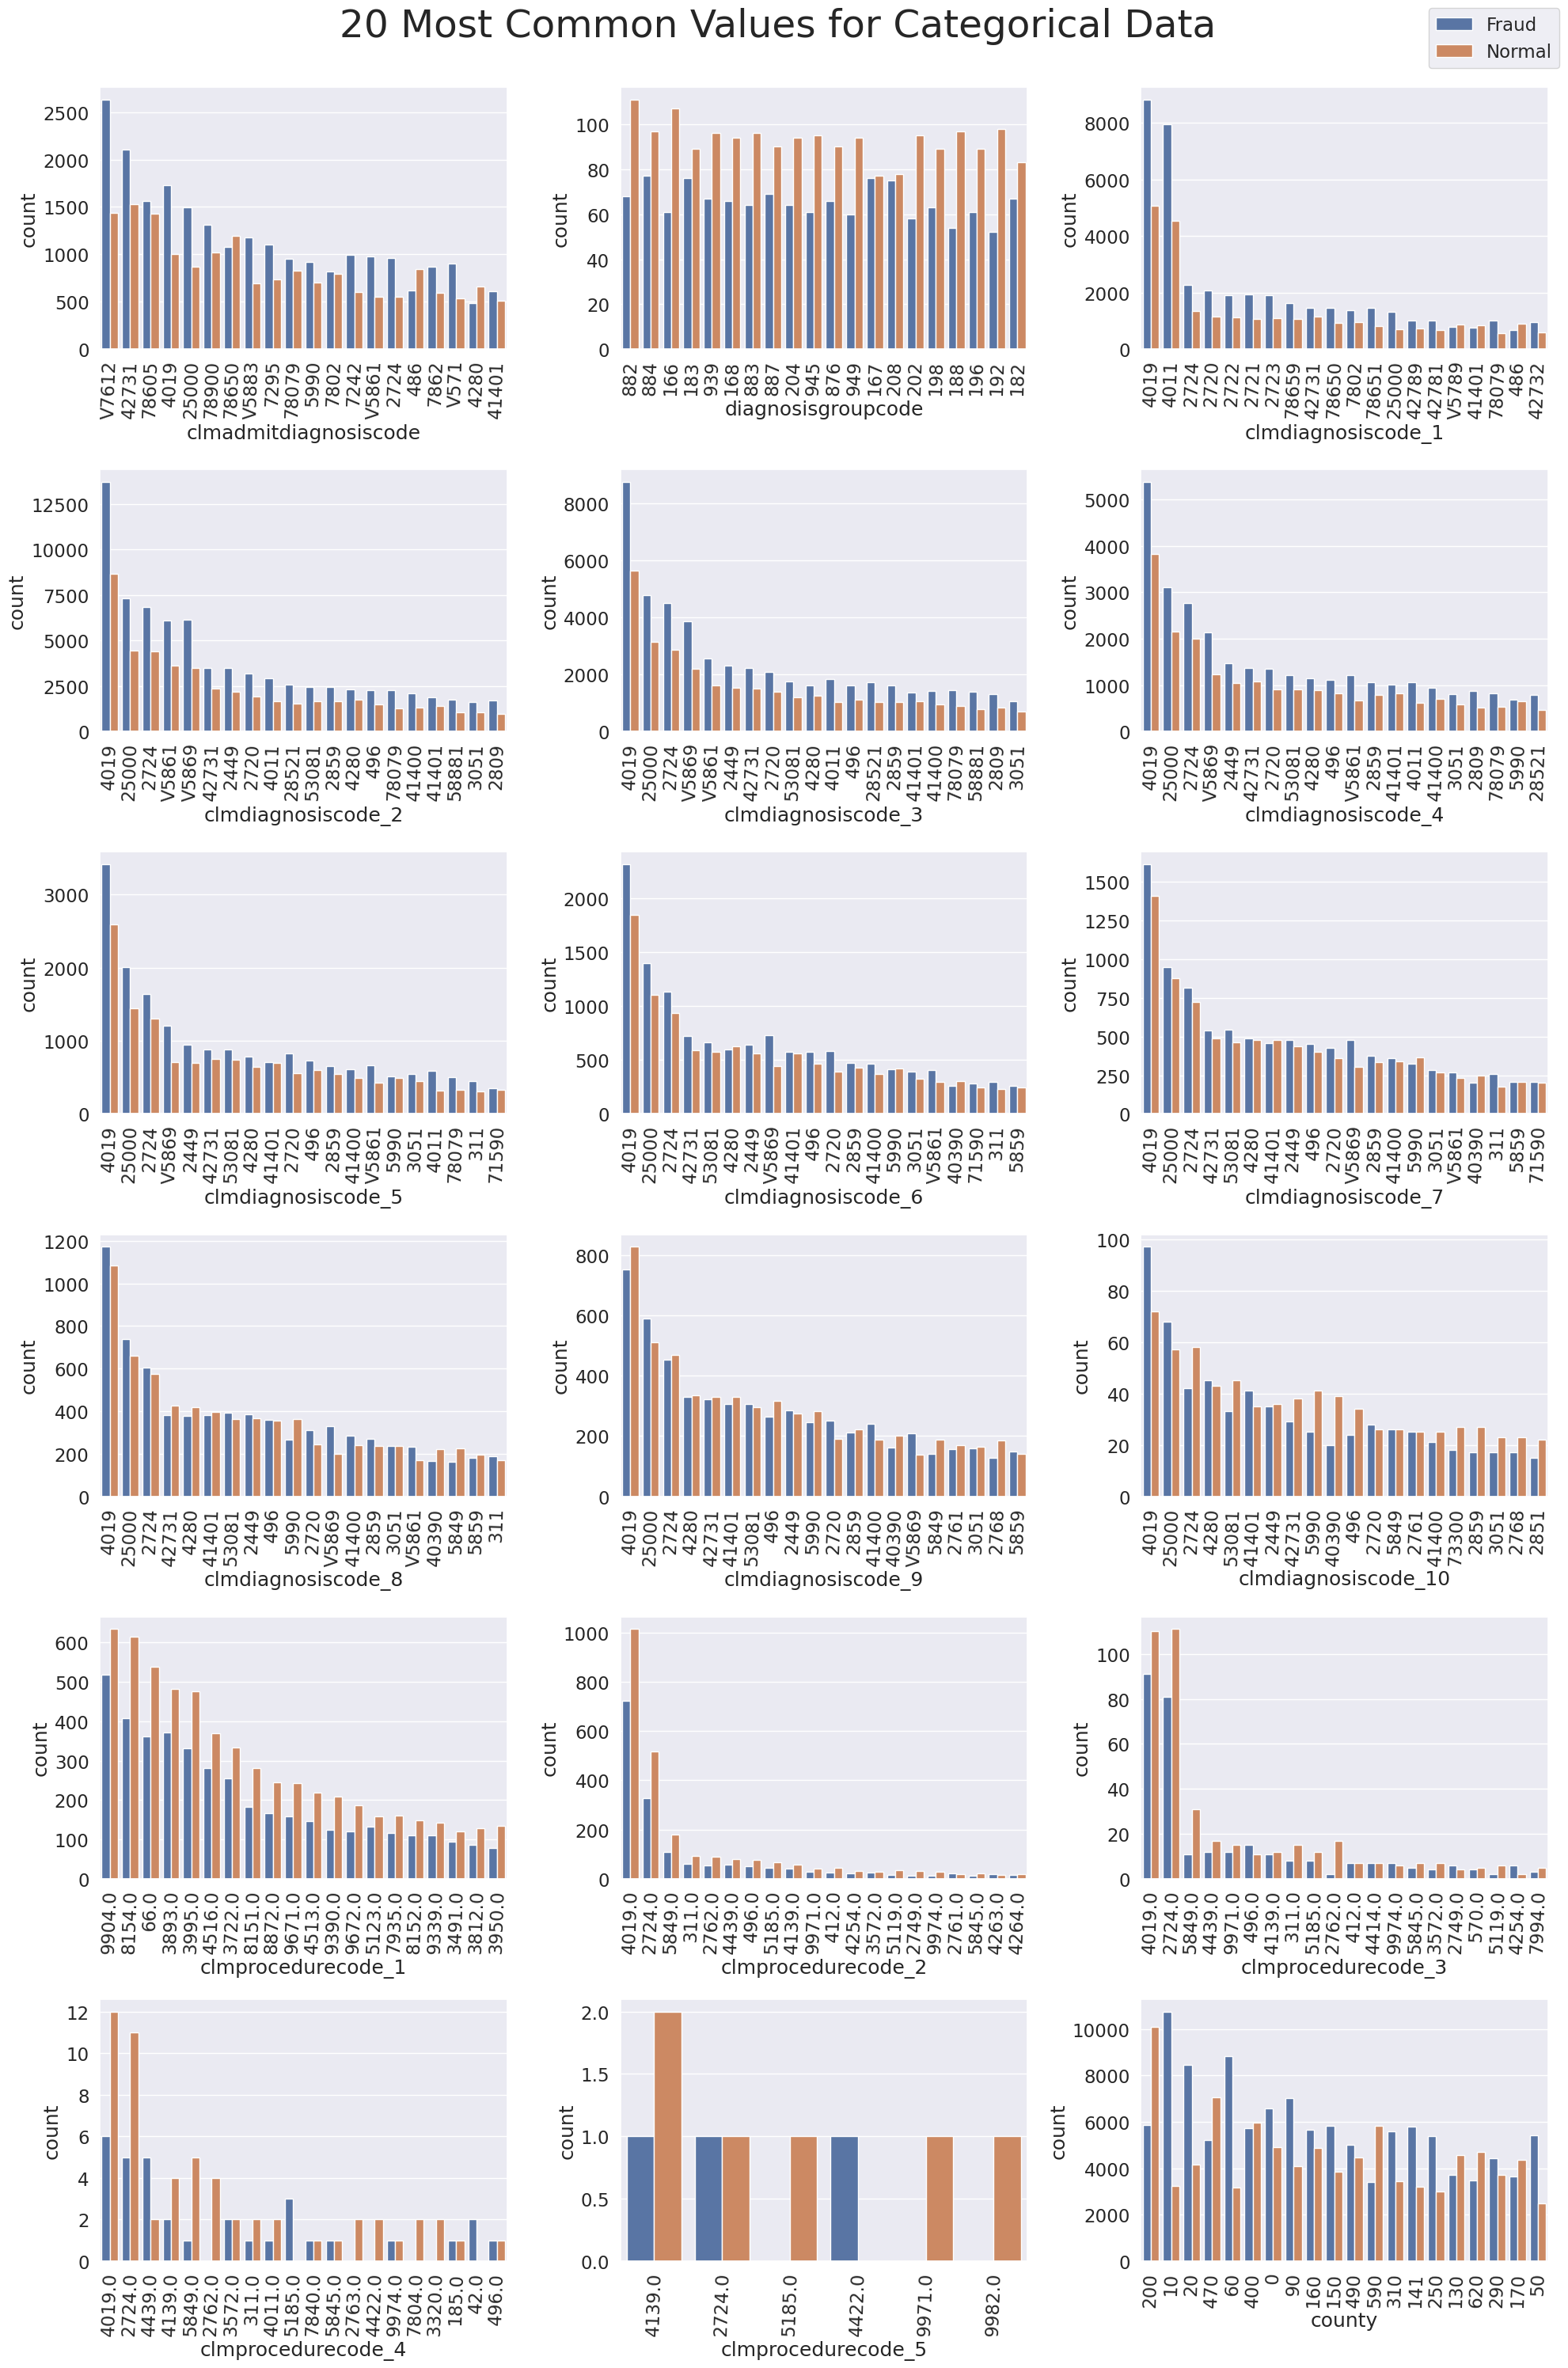
\includegraphics[width=\textwidth]{./img/categorical.png}
  \caption{20 Most Common Values for Categorical Data}
  \label{fig:categorical}
\end{figure}

\newpage
To analyze the quantitative data, the boxplots are generated (Figure 7). The values are normalized on a 
0-1 scale. The plots show that certain attributes are extremely concentrated and include
a number of outliars, such as deductibleamtpaid.
\begin{figure}[!htbp]
  \centering
  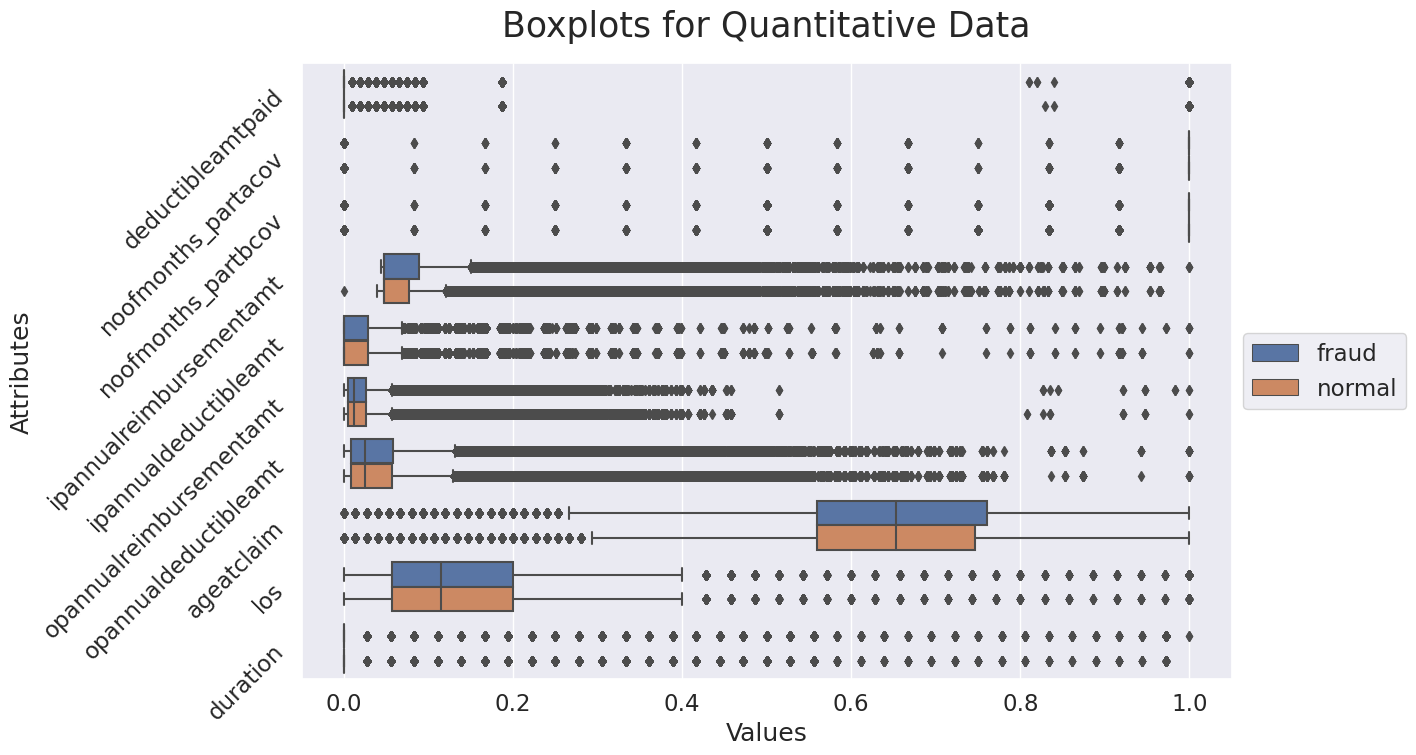
\includegraphics[width=\textwidth]{./img/boxplot.png}
  \caption{Boxplots for Quantitative Data}
\end{figure}
\newpage

PCA is applied in Figure 9,
and a subset of the data is plotted in three space.
\begin{figure}[!htbph]
  \centering
  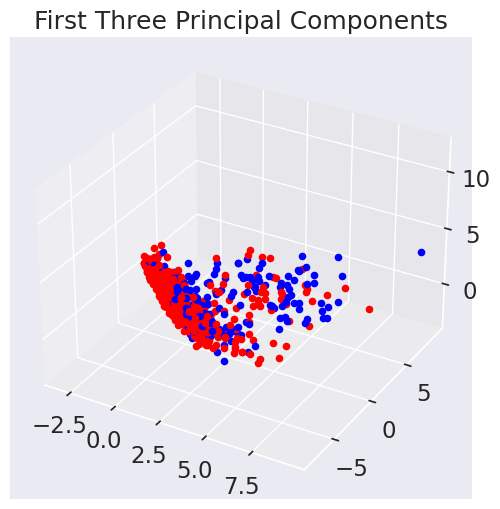
\includegraphics[width=12cm]{./img/pca.png}
  \caption{First three principal components of binary and quantitative data.
  The class of data is separated in blue and red. A degree of clustering
  is observed, meaning these features are predictive.}
\end{figure}
\newpage
A heatmap of the first three principal components is plotted.  Lighter colors imply A
positive correlation, and dark colors show a negative correlation. Either can 
demonstrate that the feature is predictive.
\begin{figure}[!htbp]
  \centering
  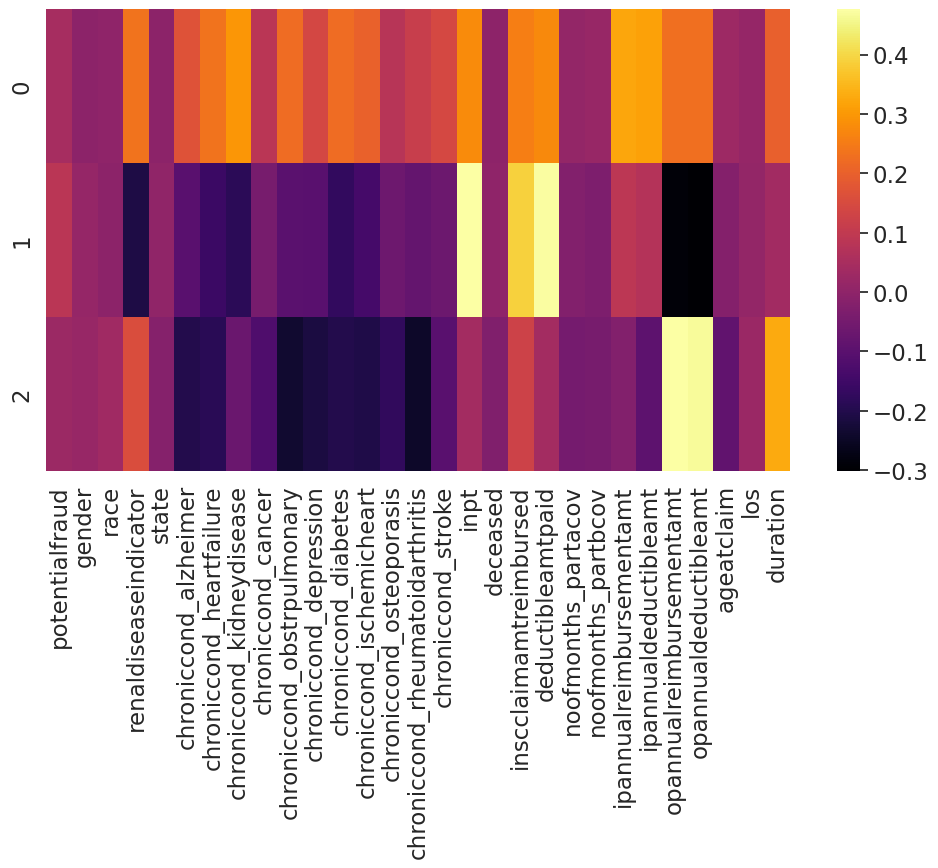
\includegraphics[width=\textwidth]{./img/pca2.png}
  \caption{Colorbar of principal components}
\end{figure}
\newpage

The correlation between quantitative features is investigated in the following
chart. A pair of features that are highly correlated with each other can suggest
that only one of the features is needed. In this case, duration and los appear
to be redundant. However, because of the PCA results (Figure 10), both features will be kept.
\begin{figure}[!htbp]
  \centering
  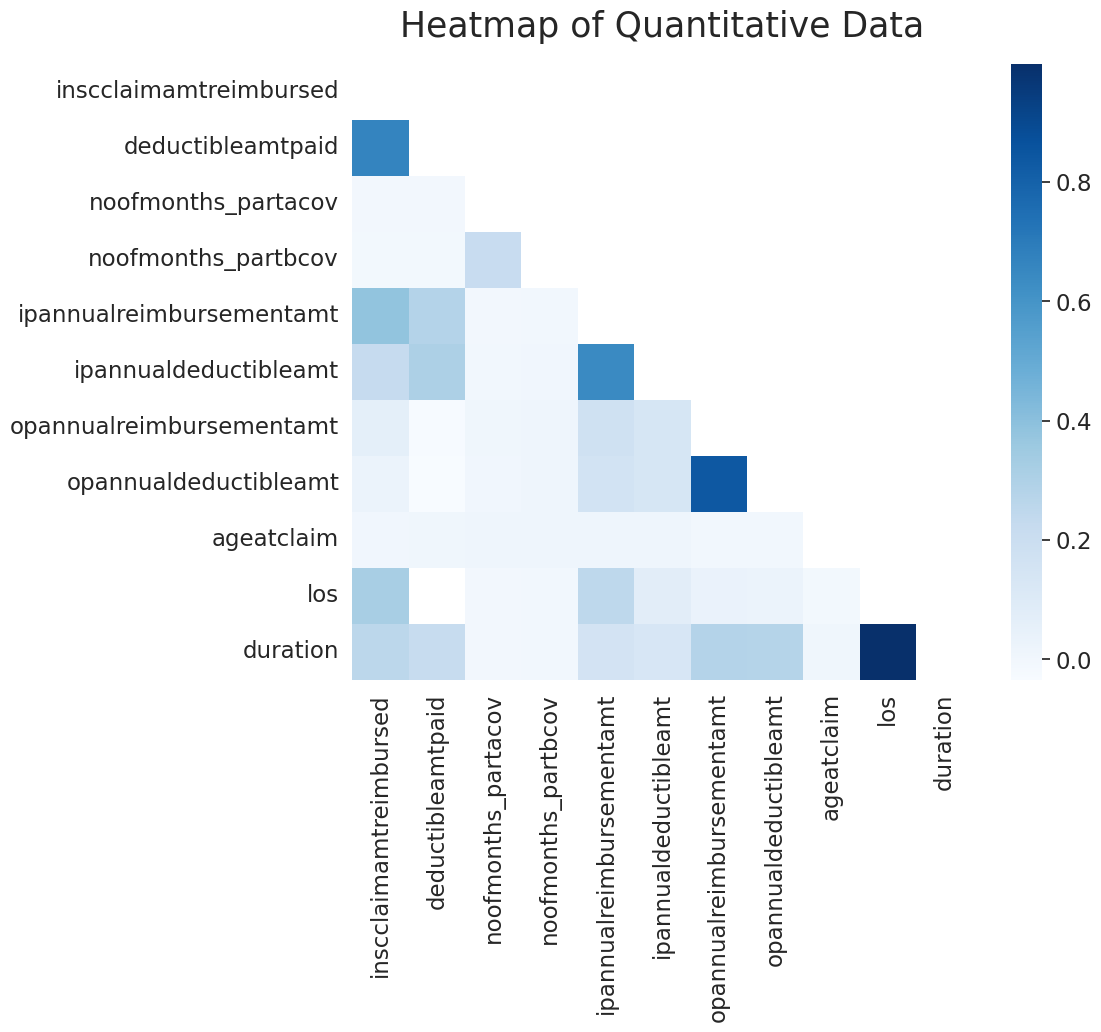
\includegraphics[width=\textwidth]{./img/heatmap.png}
  \caption{Heatmap for Quantitative Data. Darker colors show
  the feature pairs are more highly correlated}
\end{figure}
\newpage
The following scatter (figure 12) plot shows the relationship between the 
number of physicians and the percentage of fraudulent claims. 
The vertical lines on the plot indicate the number of physicians at 
which the percentage of fraudulent claims reaches 80\%, 90\%, and 99\%.

The plot suggests that a relatively small number of
physicians are responsible for a large proportion of fraudulent claims. 

\begin{figure}[!htbp]
  \centering
  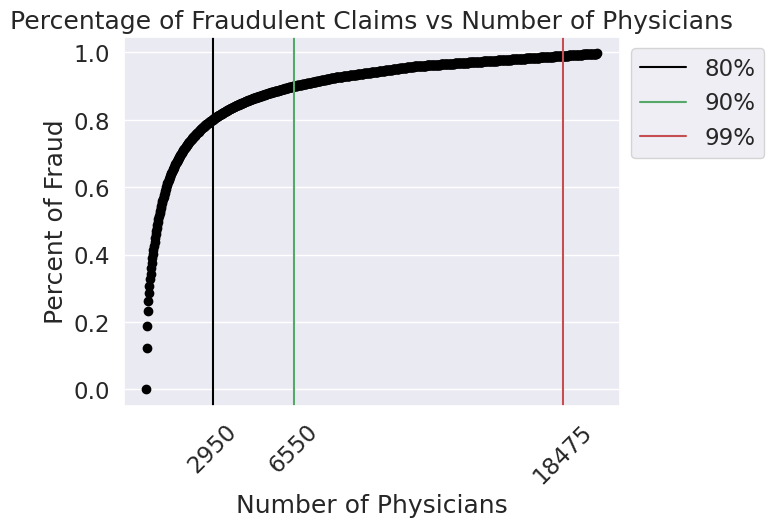
\includegraphics[width=\textwidth]{./img/fraud.png}
  \caption{The percentage of fraudulent claims vs number of physicians
  At the black vertical line, the first 2950 
  physicians with the most fraudulent claims account for 80\% of all fraudulent
  claims. This represents just 0.53\% of all physicians}
\end{figure}
\clearpage

% Preprocessing
\section{Preprocessing}

 After observing the dataset, we find only the train dataset has the label
 (fraudulent or not). Therefore, we choose to use the train dataset and 
 split the dataset into train and validation sets later. 
Firstly, we import all datasets, we use the function named col\_header\_clean
 to switch all characters in columns to lowercase, remove spaces and special chars.
  Then, to make the training set ML processible, we merge the datasets into one. 
  The inpatient and outpatient sets have similar features, so they can be merged.

  An inpatient indicator column will be created to distinguish inpatient and 
   outpatient claims. Then, values of binary categorical variables (
    'Y'/'N' or '1'/'2') are converted to 1 and 0. Also, values with 
    date and time data will be converted to the correct form. Based on the dates, 
    we also calculate information such as the patient's age at the time of claim, 
    duration of the claim, and length of hospital stay. Finally, we remove features
    having no records, and add derived features including total count of claims filed
    by physicians and total number of physicians for each provider.

\clearpage
% Models and Training
\section{Models and Training}
The following classifiers were evaluated. Out of the parameters tested, the ones provided
here yielded the best performance.
\begin{itemize}[noitemsep]
  \item  Adaboost Classifier
  \begin{itemize}[noitemsep]
    \item n\_estimators=100
  \end{itemize}
  \item  Extra Trees Classifier
  \begin{itemize}[noitemsep]
    \item n\_estimators=100
  \end{itemize}
  \item  Gradient Boosting Classifier
  \begin{itemize}[noitemsep]
    \item n\_estimators=1000
    \item max\-depth=8
  \end{itemize}
  \item  K Nearest Neighbors
  \begin{itemize}[noitemsep]
    \item n=3
  \end{itemize}
  \item  Random Forest Classifier
  \begin{itemize}[noitemsep]
    \item n\_estimators=1000
  \end{itemize}
\end{itemize}
The performance of each classifier is summarized in table 1-5.

\begin{table}[!htbp]
  \centering
  \caption{Adaboost Classifier Scores}
  \csvautotabular{csv/Adaboost.csv}
\end{table}
\vspace{-2em}
\begin{table}[!htbp]
  \centering
  \caption{Extra Trees Classifier Scores}
  \csvautotabular{"csv/Extra Trees.csv"}
\end{table}
\vspace{-2em}
\begin{table}[!htbp]
  \centering
  \caption{Gradient Boosting Classifier Scores}
  \csvautotabular{"csv/Gradient Boosting.csv"}
\end{table}
\vspace{-2em}
\begin{table}[!htbp]
  \centering
  \caption{K Nearest Neighbors Scores (n=3)}
  \csvautotabular{csv/KNN.csv}
\end{table}
\vspace{-2em}
\begin{table}[!htbp]
  \centering
  \caption{Random Forest Scores}
  \csvautotabular{"csv/Random Forest.csv"}
\end{table}
\newpage

The receiver operating characteristic curve is plotted for the algorithms.

\begin{figure}[!ht]
  \centering
  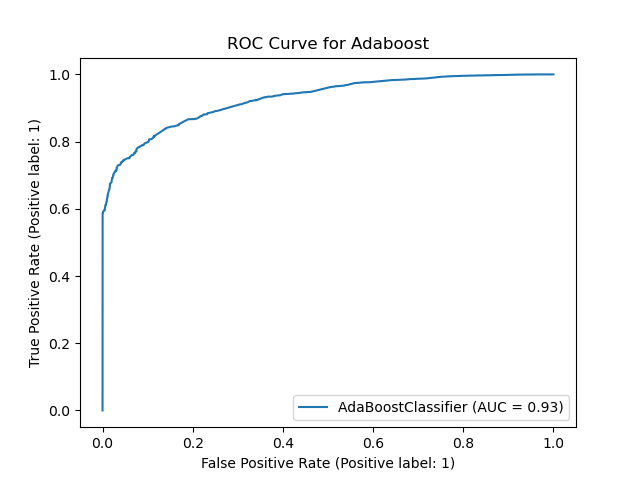
\includegraphics[width=11.5cm]{./img/AdaboostROC.png}
  \caption{ROC curve for Adaboost Classifier}
\end{figure}
\begin{figure}[!ht]
  \centering
  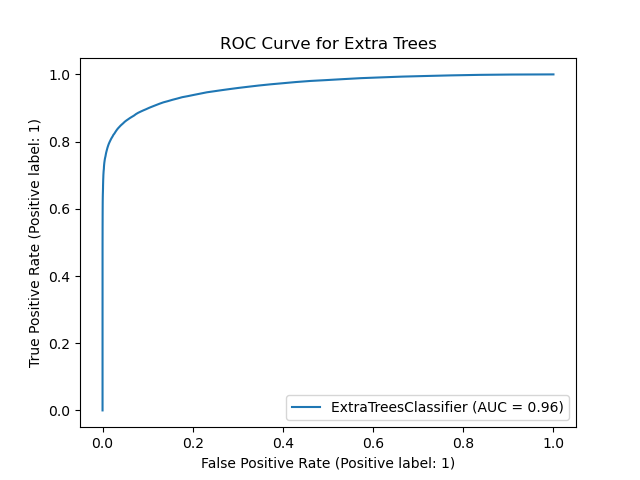
\includegraphics[width=11.5cm]{./img/ExtraTreesROC.png}
  \caption{ROC curve for extra trees classifier}
\end{figure}
\begin{figure}[!ht]
  \centering
  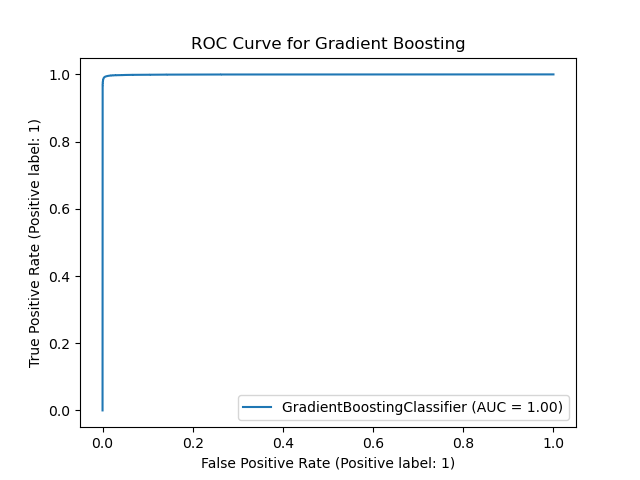
\includegraphics[width=11.5cm]{./img/GradientBoostingROC.png}
  \caption{ROC curve for gradient boosting classifier}
\end{figure}
\begin{figure}[!ht]
  \centering
  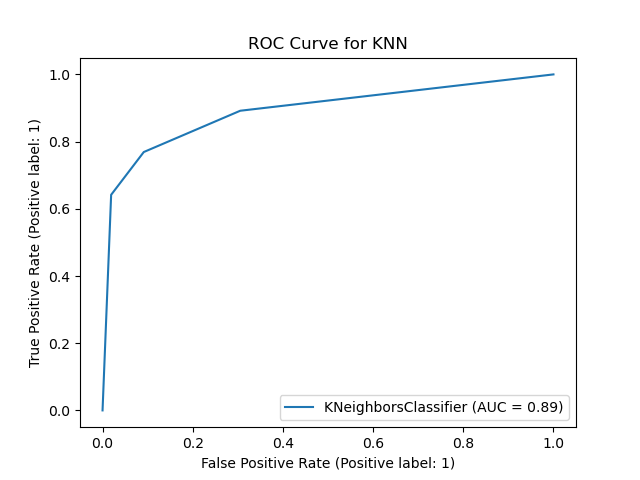
\includegraphics[width=11.5cm]{./img/KNNROC.png}
  \caption{ROC curve for KNN classifier}
\end{figure}
\clearpage
\begin{figure}[!ht]
  \centering
  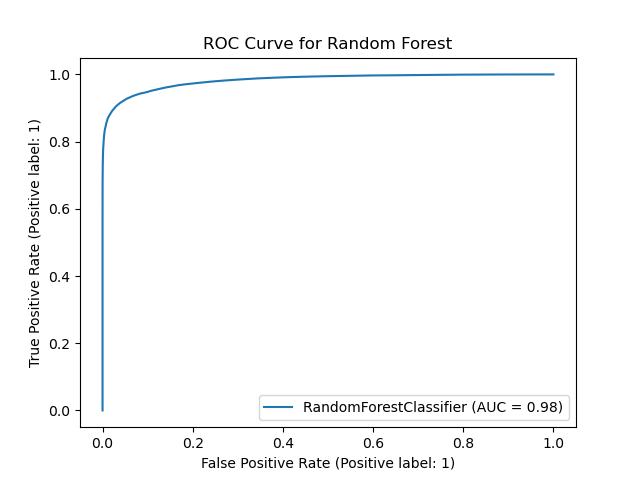
\includegraphics[width=11.5cm]{./img/RandomForestROC.png}
  \caption{ROC curve for Random Forest classifier}
\end{figure}
The gradient boosting classifier outperformed the other algorithms on all metrics, 
while achieving an area under the curve of nearly 1.00. Because of its excellent
ROC Curve, f1-score, precision, and recall, this classifier was selected for use.
\clearpage
A streamlit application was developed to allow users to interact with the selected model.
The application is hosted
\href{https://dmt-final-proj.streamlit.app/}{here}.
Streamlit offers a framework for developing user interfaces for machine learning models
as well as a web hosting service. The hosing services requires developers to provide
streamlit access to a github repository and a configuration file.
Github allows users to upload files of size 50MB for free. This served as an additional
constraint when deploying this service. The random forest classifier had a size of 0.5GB,
and even after compression, it was far too large. Fortunately, the gradient boosting 
classifier required 0.12 MB of storage. The storage size of this classifier is sensitive
to the maximum depth, and not to the number of classifiers.
The user interface is presented in the next section:

\begin{figure}[h]
  \centering
  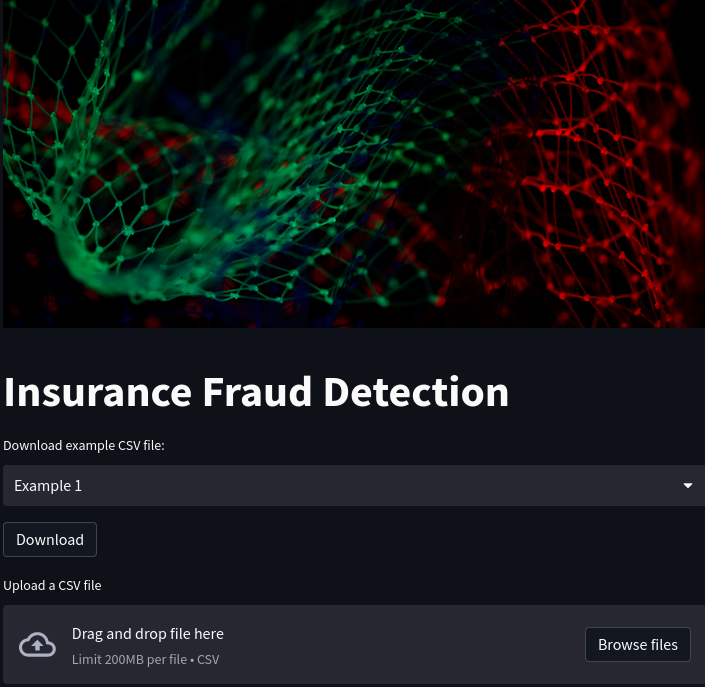
\includegraphics[width=\textwidth]{./img/streamlit.png}
  \caption{Graphical user interface for Streamlit service}
\end{figure}
The user can download example data from the application for testing purposes.
The CSV can serve as a template for users to fill out with their own data. 
The upload section allows users to input up to 200MB of data to be classified.
\begin{figure}[!ht]
  \centering
  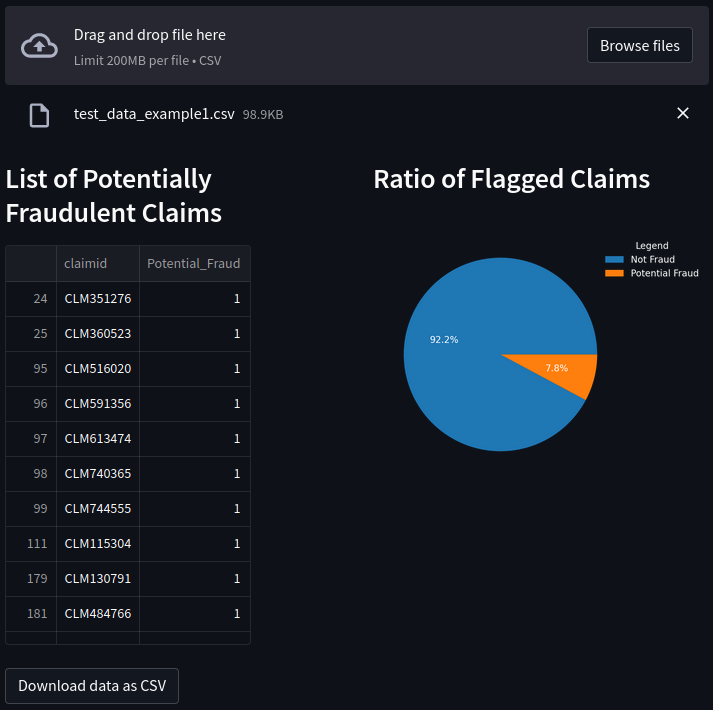
\includegraphics[width=\textwidth]{./img/streamlit2.png}
  \caption{Example output}
\end{figure}
As seen in Figure 19, the application will produce a list of claims that are potentially
fraudulent. Users can view the table in the application, or download the data and view
with any CSV compatible application.
\begin{figure}[!ht]
  \centering
  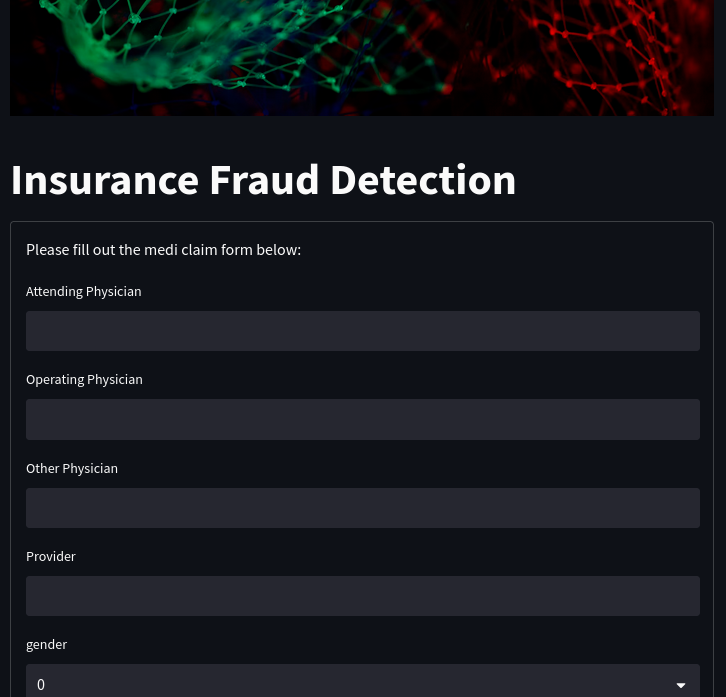
\includegraphics[width=\textwidth]{./img/streamlit3.png}
  \caption{Users can also elect to input a single data point in a fourm}
\end{figure}
\clearpage
\section{Future Enhancements}
As previously discussed, the model exhibits exceptional performance. However,
there are certainly other models that could outperform the
gradient boosted classifier. Additionally, final model was still not overfitted,
and given more time, a better performance could likely be achieved with the same classifier.




\clearpage

\section{References}
\begin{enumerate}[noitemsep]
  \item fbi.gov
  \item https://stackoverflow.com/questions/45003577/how-to-output-classification-report-of-sklearn-into-a-csv-file
  \item https://seaborn.pydata.org/generated/seaborn.displot.html
  \item https://www.kaggle.com/datasets/beenusharma42/fraudlent-claim-in-healthcare
  \item https://scikit-learn.org/stable/modules/generated/sklearn.metrics.roc\_curve.html
  \item https://scikit-learn.org/stable/auto\_examples/model\_selection/plot\_det.html\#sphx-glr-auto-examples-model-selection-plot-det-py
  \item https://seaborn.pydata.org/generated/seaborn.heatmap.html
  \item https://seaborn.pydata.org/examples/horizontal\_boxplot.html
  \item https://scikit-learn.org/stable/modules/generated/sklearn.ensemble.RandomForestClassifier.html
  \item https://scikit-learn.org/stable/modules/generated/sklearn.metrics.classification\_report.html
  \item https://scikit-learn.org/stable/modules/generated/sklearn.ensemble.ExtraTreesClassifier.html
  \item https://scikit-learn.org/stable/modules/generated/sklearn.ensemble.AdaBoostClassifier.html
  \item https://scikit-learn.org/stable/modules/generated/sklearn.neighbors.KNeighborsClassifier.html
  \item "Introduction to Machine Learning with Python: A Guide for Data Scientists by Andreas Müller (Author), Sarah Guido (Author) "


\end{enumerate}
\end{document}